
\providecommand{\toplevelprefix}{../..}  % necessary for subfile bibliography + figures compilation to work, do not move this after documentclass
\documentclass[../../book-main_zh.tex]{subfiles}

\begin{document}

\chapter{智能研究的未来}
\label{ch:future}

% \begin{quote}
% ``{\em If I were to choose a patron saint for cybernetics
% out of the history of science, I should have to choose
% Leibniz. The philosophy of Leibniz centers about two
% closely related concepts -- that of a universal symbolism
% and that of a calculus of reasoning.}''

% $~$\hfill -- Norbert Wiener, Cybernetics, 1961
  
% \end{quote}

\begin{quote}
“{\em 这项研究将基于一个猜想展开,即学习的每一个方面或智能的任何其他特征,原则上都可以被精确地描述,从而可以用一台机器来模拟它。我们将尝试找出如何让机器使用语言、形成抽象和概念、解决目前只有人类才能解决的各种问题,并进行自我改进。}”

$~$\hfill —— 达特茅斯人工智能项目提案,1956年
 \end{quote}
\vspace{5mm}

%This chapter discusses active ongoing research topics on intelligence as well as some challenges and opportunities for future study.

总的来说,本书稿旨在系统地介绍如何从经验观察中发展记忆或知识的数学原理和计算机制。在一个看似随机的世界中寻求简约性的能力,是任何智能(无论是自然的还是人造的)的基本特征。我们相信,本书中提出的原理和机制是相当统一和普适的,既适用于动物,也适用于机器。

我们希望本书能帮助读者透彻地揭开现代人工深度神经网络实践的神秘面纱,通过对其功能和作用——即服务于从高维数据中学习低维分布这一目标——建立严谨的理解。有了这样的理解,我们应该能意识到现有AI模型和系统的能力与局限:
\begin{enumerate}
    \item 就一个能够自我学习和自我完善的记忆系统而言,现有的模型和系统尚不完备。
    \item 在学习策略和优化技术方面,对这些功能的现有实现仍然相当原始和粗放,远非最优。
    \item 现有方法仅学习经验数据分布并对其进行归纳推理,这与高阶的人类智能有所不同。
\end{enumerate} 

本书的目标之一是帮助人们对当前的机器智能技术建立客观的理解,并认识到智能研究未来仍然面临哪些开放性问题和挑战。在本书的最后一章,我们将就未来提供一些我们的观点和展望。

\section{迈向自主智能:闭环学习?}
从过去十年机器智能的实践中可以清楚地看到,只要有足够的数据和计算资源,人们就可以构建一个足够大的模型,并对其进行预训练,以学习所有数据的\textit{先验}分布,例如$p(\x)$。理论上,这样一个大型模型几乎可以记住所有已编码于海量语言和文本中的关于世界的现有知识。正如我们在本书开头所讨论的,在某种程度上,这种大型模型扮演着与DNA相似的角色,生命利用DNA来记录和传递关于世界的知识。

然后,这个学习到的模型和分布可以被用来基于相同的分布重新生成新的数据样本。人们也可以利用该模型,在各种条件下,利用记忆的知识进行推理(例如,估计、预测),比如说在有新观测$\y$的情况下,通过对\textit{后验}分布$p(\x\mid \y)$进行采样。严格来说,这种推理是统计性的。

然而,任何预训练模型,无论多大,都不能保证它迄今为止学到的分布是完全正确或完备的。万一我们从当前的\textit{先验}分布$p_t(\x)$中抽取的样本$\hat{\x}_t$,或基于\textit{后验}分布$p_t(\x\mid \y)$的估计$\hat{\x}_t(\y)$与真实值$\x$不一致,我们就非常希望能修正已学习的分布:
\begin{equation}
    p_t(\x) \rightarrow p_{t+1}(\x) \quad \mbox{或}\quad p_t(\x\mid \y) \rightarrow p_{t+1}(\x\mid \y),
\end{equation}
这需要基于误差$\boldsymbol{e}_t = \x_t - \hat{\x}_t$。这被称为基于误差反馈的纠错,是自然界中一种无处不在的、用于持续学习的机制。然而,正如我们所知,任何开放式模型本身都不具备在所学分布不正确或不完备时对其进行修正或改进的机制。改进当前的AI模型在很大程度上仍然依赖于人类的参与:实验、评估和选择。我们可以将这个过程称为大型模型的“人工选择”,以区别于生命演化中的自然选择。

正如我们在本书前面(特别是第\ref{ch:closed-loop}章)所研究的,闭环系统能够将内部表征与外部世界的(感知)观测对齐。它可以持续改进内部学习到的分布及其表征,以实现一致性或自洽性。未来的一个直接步骤是开发和构建真正的闭环记忆系统,如图\ref{fig:open-to-closed}所示,这些系统能够基于误差反馈,自主、持续地学习和改进更通用的数据分布。

因此,从当前流行的端到端训练的开环模型过渡到持续学习的闭环系统:
\begin{equation}
   \mbox{\textbf{开环}模型} \; \Longrightarrow \; 
   \mbox{\textbf{闭环}系统}
\end{equation}
是让机器真正模拟(动物)大脑如何在开放世界中学习和应用知识的关键。我们相信:
\begin{quote}
\begin{center}
        {\em 开环模型适用于封闭世界,无论其多么大; \\ 闭环系统则适用于开放世界,无论其多么小。}
\end{center}
\end{quote}
事实上,“通用智能”绝不可能仅仅通过记忆世界上所有现存的知识来实现。相反,通用智能只能通过拥有改进其现有记忆的机制来实现,从而能够适应任何新的环境和任务。

\begin{figure}[t]
    \centering    
    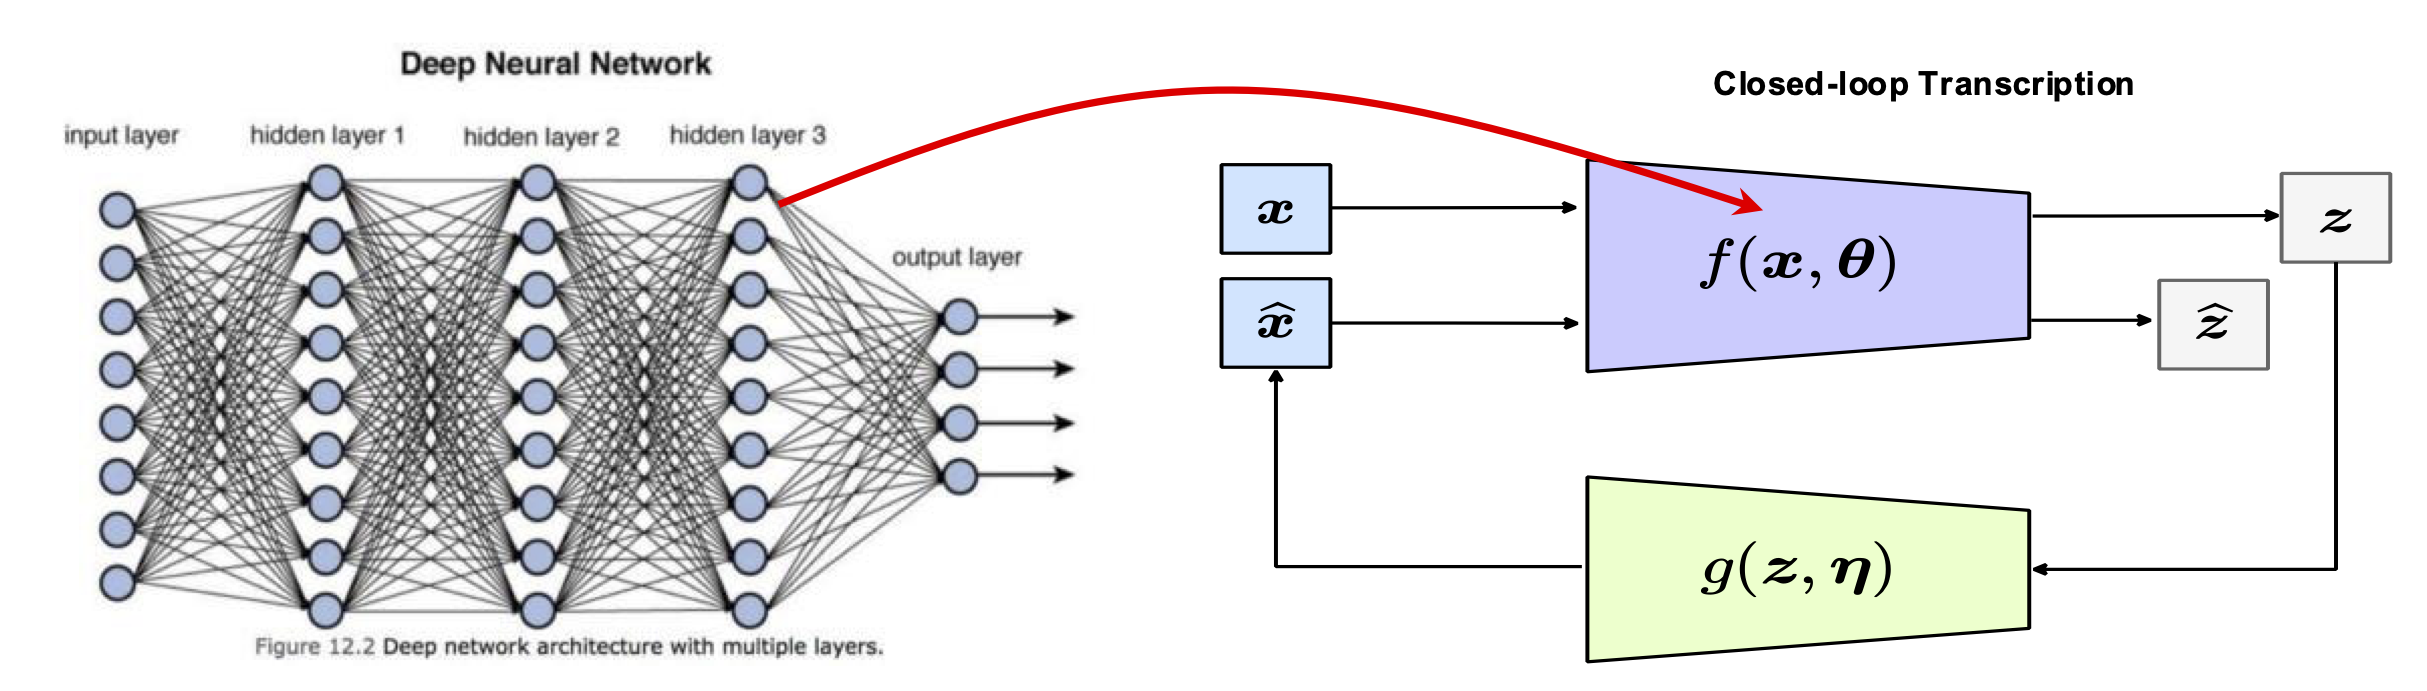
\includegraphics[width=0.9\linewidth]{\toplevelprefix/chapters/chapter8/figs/open-to-closed.png}
    \caption{从开环深度网络到闭环系统。}
    \label{fig:open-to-closed}
\end{figure}



\section{迈向自然智能:超越反向传播?}
过去几年机器智能的实践让许多人相信,我们需要构建一个单一的大型模型来学习所有数据的分布并记忆所有知识。即使这在技术上是可行的,这样的解决方案很可能远非必要和高效。正如我们从训练深度网络的实践中所知,唯一已知能大规模训练此类网络的方法是通过反向传播(BP)\cite{Back-Prop}。尽管BP提供了一种通过在整个模型中反向传播梯度信号来纠正错误的方法,但它仍然相当粗放,并且与自然界的学习方式有显著不同:BP是一个自然界因其高昂成本而无法承受,或因物理限制而根本无法实现的选项。

更普遍地说,除非我们同时理解智能如何被高效地实现,否则我们无法真正理解智能。也就是说,我们需要解决实现与智能目标相关的机制的计算复杂性问题。值得注意的是,历史上,我们对(机器)智能的理解正是经历了几个阶段的演变,从不可计算的柯尔莫哥洛夫复杂性到香农熵,从图灵的可计算性到后来对可处理性\footnote{如果一个问题允许一个其复杂度是问题规模的多项式的算法,我们就说这个问题是可处理的。}的理解,再到现代人工智能实践中对算法可扩展性的强烈重视。这一演变可以概括为以下图示:
\begin{equation}
   \mbox{\textbf{不可计算}} \;
   \Longrightarrow \; \mbox{\textbf{可计算}} \;
   \Longrightarrow \; \mbox{\textbf{可实现}} \; \Longrightarrow \; 
   \mbox{\textbf{可扩展}}。
\end{equation}
在很大程度上,深度学习和反向传播的成功与普及,恰恰是因为它们为处理和压缩海量数据提供了在现代计算平台(如GPU)上可扩展的实现。然而,与自然界实现智能的方式相比,这种实现的成本仍然高得太多。

机器智能的效率仍有巨大的提升空间,以期能够模拟自然智能的效率水平,后者应比当前粗放的实现方式高出几个数量级。为此,我们需要发现新的学习架构和优化机制,这些机制能够在自然的物理条件和资源约束下学习数据分布,类似于自然界中智能生物所面临的那些约束,例如,无需一次性访问所有数据,或一次性(通过BP)更新所有模型参数。

本书中阐述的原则性框架和方法可以引导我们去发现这样的新架构和机制。这些新架构和机制应该能够实现线上的持续学习,并且可以通过高度局部化和稀疏的前向或后向优化进行更新。到目前为止,对于学习一个分布,我们唯一知道存在这种解的最简单情况是主成分分析(PCA),其在线PCA方法已在第\ref{ch:autoencoding}章中介绍。

\begin{figure}[t]
\centering
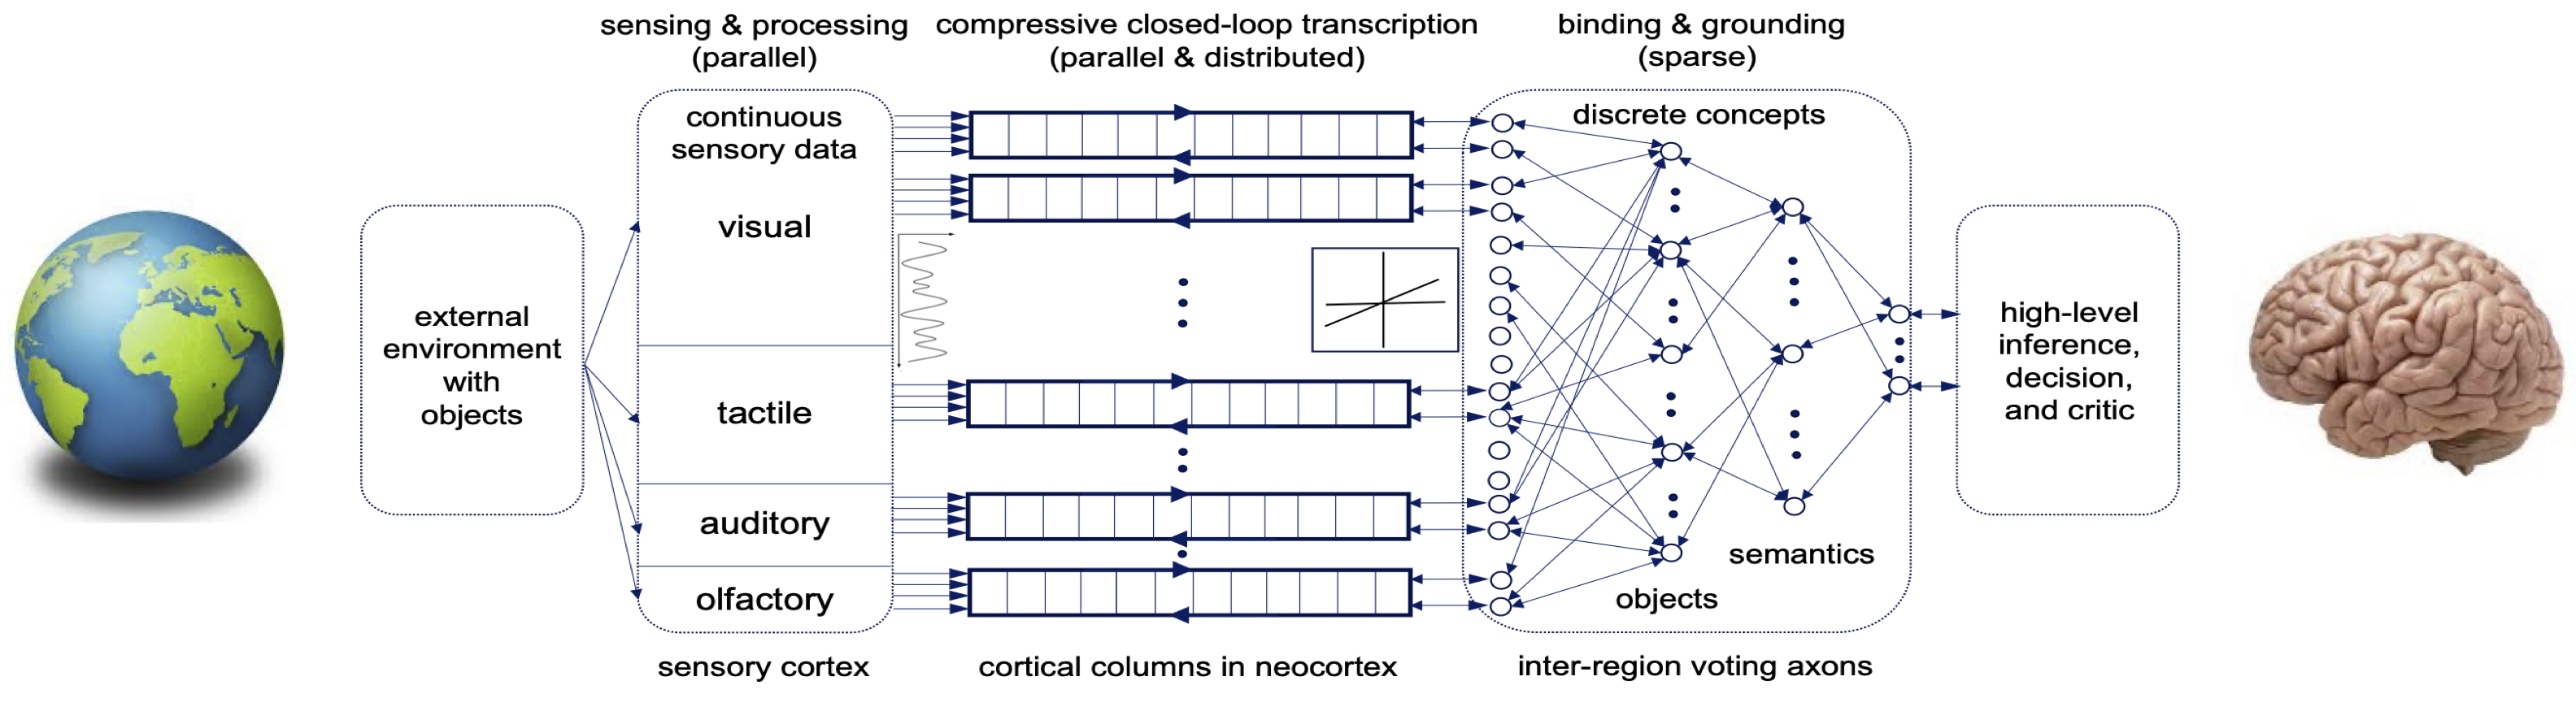
\includegraphics[width=0.99\linewidth]{\toplevelprefix/chapters/chapter8/figs/loops.png}
    \caption{大脑皮层的推测架构:皮层是一个大规模并行和分布式的自编码系统,由一系列分层的闭环自编码器组成。这些自编码器从多种感官中提取信息,并在多个层次和粒度上最大化所生成表征的信息增益。}
    \label{fig:loops}
\end{figure}
正如我们从神经科学中所了解的,我们大脑的皮层由数万个皮层柱组成。所有的皮层柱都具有相似的物理结构和功能。它们是高度并行和分布式的,尽管连接是稀疏的。因此,我们相信,为了开发一个更具可扩展性和结构化的记忆系统,我们需要考虑模拟皮层那样的架构。图\ref{fig:loops}展示了这样一个假设的架构,一个大规模分布式和分层的系统,由许多基本并行的闭环自编码模块组成。这些模块学习编码不同的感觉模态,或来自每个感觉模态的数据的许多投影。我们在第\ref{ch:conditional-inference}章第\ref{sec:measurement-self-consistency}节的讨论表明,这种并行感知和学习低维分布在理论上是可能的。更高层的(有损)自编码器则可以在低层自编码器的输出基础上进行学习,以发展出更稀疏、更高级别的对低层所学表征的“抽象”。

图\ref{fig:loops}所示的分布式、分层和闭环的系统架构与大脑皮层的许多特征相吻合。这样的系统架构可能比当前单一大型模型的架构开辟更多的可能性。它使得探索更高效的学习和优化机制成为可能,并能产生更具结构化、模块化的对所学数据分布和知识的组织。这将使我们能够将机器智能的实现带到下一个演化阶段:
\begin{equation}
   \mbox{\textbf{不可计算}} \;
   \Longrightarrow \; \mbox{\textbf{可计算}} \;
   \Longrightarrow \; \mbox{\textbf{可实现}} \; \Longrightarrow \; 
   \mbox{\textbf{可扩展}} \; \Longrightarrow \; 
   \mbox{\textbf{自然}}。
\end{equation}

\section{迈向人类智能:超越图灵测试?}
正如我们在本书开篇(第\ref{ch:intro}章)所讨论的,自然界的智能也经历了多个发展阶段,并至少以四种不同形式显现:
\begin{equation}
\mbox{\textbf{物种智能}} \;
   \Longrightarrow \; \mbox{\textbf{个体智能}} \; \Longrightarrow \; 
   \mbox{\textbf{社会智能}}
   \; \Longrightarrow \; 
   \mbox{\textbf{人工智能}}。
\end{equation}
尽管所有形式的智能都共享学习关于世界的有用知识这一共同目标,但它们在具体的编码方案、所编码的信息、学习和改进的计算机制以及这些机制的物理实现上可能表现出显著的差异。使用本书中发展的概念和术语,从学习和表示感知数据分布中信息的角度来看,这四个智能阶段在以下三个方面有所不同:
\begin{itemize}
    \item 用来学习和编码目标信息或知识的码本。
    \item 使用该码本存储和表示的信息或知识。
    \item 用于改进信息和知识的计算或优化机制。
\end{itemize}
更具体地说,下表总结了它们在上述三个方面的主要特征:
\begin{center}
%\begin{small}
\begin{tabular}{| c | c | c | c | c |}
\hline & \textbf{物种智能} & \textbf{个体智能} & \textbf{社会智能} & \textbf{人工智能}\\
\hline
\textbf{编码语言}  & 氨基酸 & 神经元 & 字母与词汇 & 数学/逻辑 \\ [0.5ex]
  \hline 
\textbf{记录信息} & 基因/DNA & 记忆 & 语言/文本 & 科学事实\\ [0.5ex]
  \hline
\textbf{优化机制} & 强化学习 & 误差反馈 & 试错法 & 假设检验 \\  [0.5ex]
\hline
\end{tabular}
%\end{small}
\end{center}


% \begin{equation}
% \mbox{\textbf{Amino Acids}} \;
%    \Longrightarrow \; \mbox{\textbf{Brain}} \; \Longrightarrow \; 
%    \mbox{\textbf{Languages}}
%    \; \Longrightarrow \; 
%    \mbox{\textbf{Mathematics \& Logic}}.
% \end{equation}

% \begin{equation}
% \mbox{\textbf{Genes}} \;
%    \Longrightarrow \; \mbox{\textbf{Memory}} \; \Longrightarrow \; 
%    \mbox{\textbf{Books}}
%    \; \Longrightarrow \; 
%    \mbox{\textbf{Science}}.
% \end{equation}

% \begin{equation}
% \mbox{\textbf{RL}} \;
%    \Longrightarrow \; \mbox{\textbf{Feedback}} \; \Longrightarrow \; 
%    \mbox{\textbf{Empirical}}
%    \; \Longrightarrow \; 
%    \mbox{\textbf{Hypotheses Testing}}.
% \end{equation}


众所周知,人类在历史上实现了两次智能质的飞跃。第一次是大约五千到一万年前口头和书面语言的发展。这使得人类能够分享和传承世代积累的知识,其作用类似于自然界中的DNA。第二次是大约三千年前数学和逻辑的发展,它们已成为现代科学的精确语言。这种新语言使我们摆脱了以经验形式从观察中总结知识的束缚,允许我们将知识形式化为可通过数学推导或实验验证来证实或证伪的理论。通过提出假设、逻辑推导和实验测试,我们能够主动发现以前通过被动学习数据分布不可能发现的新知识\footnote{例如因果关系}。

正如我们在引言(第\ref{ch:intro}章)中讨论的,1956年的“人工智能”(AI)项目正是旨在研究那些被认为能将人类与动物区分开来的高阶功能,如数学抽象、逻辑推理和问题解决:
\begin{equation}
   \mbox{\textbf{低阶}(动物)智能} \; \Longrightarrow \; 
   \mbox{\textbf{高阶}(人类)智能。}
\end{equation}
正如我们在本书中反复阐明的,过去几十年机器智能的技术进步,尽管是在“AI”的名义下进行的,但实际上与动物和人类共有的、主要是归纳性的低阶智能更为相关。到目前为止,没有证据表明这些机制足以实现最初AI项目真正旨在理解和模拟的高阶人类智能。

事实上,尽管图灵测试自1950年\cite{Turing-1950}提出以来就已存在,但我们对于如何严格验证一个系统是否真正具备某种高阶智能知之甚少。\footnote{在图灵的提案中,评估者是人类。然而,大多数人类评估者的科学训练和知识可能有限,他们的结论也可能带有主观性。} 很长一段时间里,这样的测试被认为没有必要,因为机器的能力远低于人类(甚至动物)。然而,鉴于近期的技术进步,许多模型和系统声称已达到甚至超越了人类智能。因此,现在是时候为图灵测试给出一个科学且可执行的定义了。也就是说,我们如何系统、客观地评估一个给定模型或系统的智能水平?例如,我们如何严格验证一个智能系统是否真正掌握了某个抽象概念,比如自然数的概念,还是仅仅记住了大量的实例?请注意,最先进的大型语言模型在简单的数学问题上仍然会遇到困难,比如:“3.11比3.9大还是小?”\footnote{请注意,一些大型模型已经通过后期工程修正了对这类问题的回答。然而,我们留给读者一个练习,去严格测试任何一个最先进的语言模型是否真正理解自然数的概念及相关的算术运算。}
如何验证一个系统是真正理解了逻辑规则并知道如何严格应用它们,还是仅仅记住了大量实践逻辑的实例?此外,这样的系统是否甚至有能力纠正自己的知识,或发展出新的知识,如物理定律、数学概念或因果关系?总而言之,我们是时候开发出能够区分一个系统/模型的看似智能的能力究竟属于以下哪种情况的严格评估方法了:
\begin{enumerate}
    \item 仅仅是记住了某些承载知识的数据的分布并重新生成它们;
    \item 能够从新的观察中自主、持续地发展新知识;
    \item 真正理解了某些抽象知识并知道如何正确应用它;
    \item 能够产生新的科学假说或数学猜想并加以验证。
\end{enumerate}

\begin{figure}[t]
    \centering
    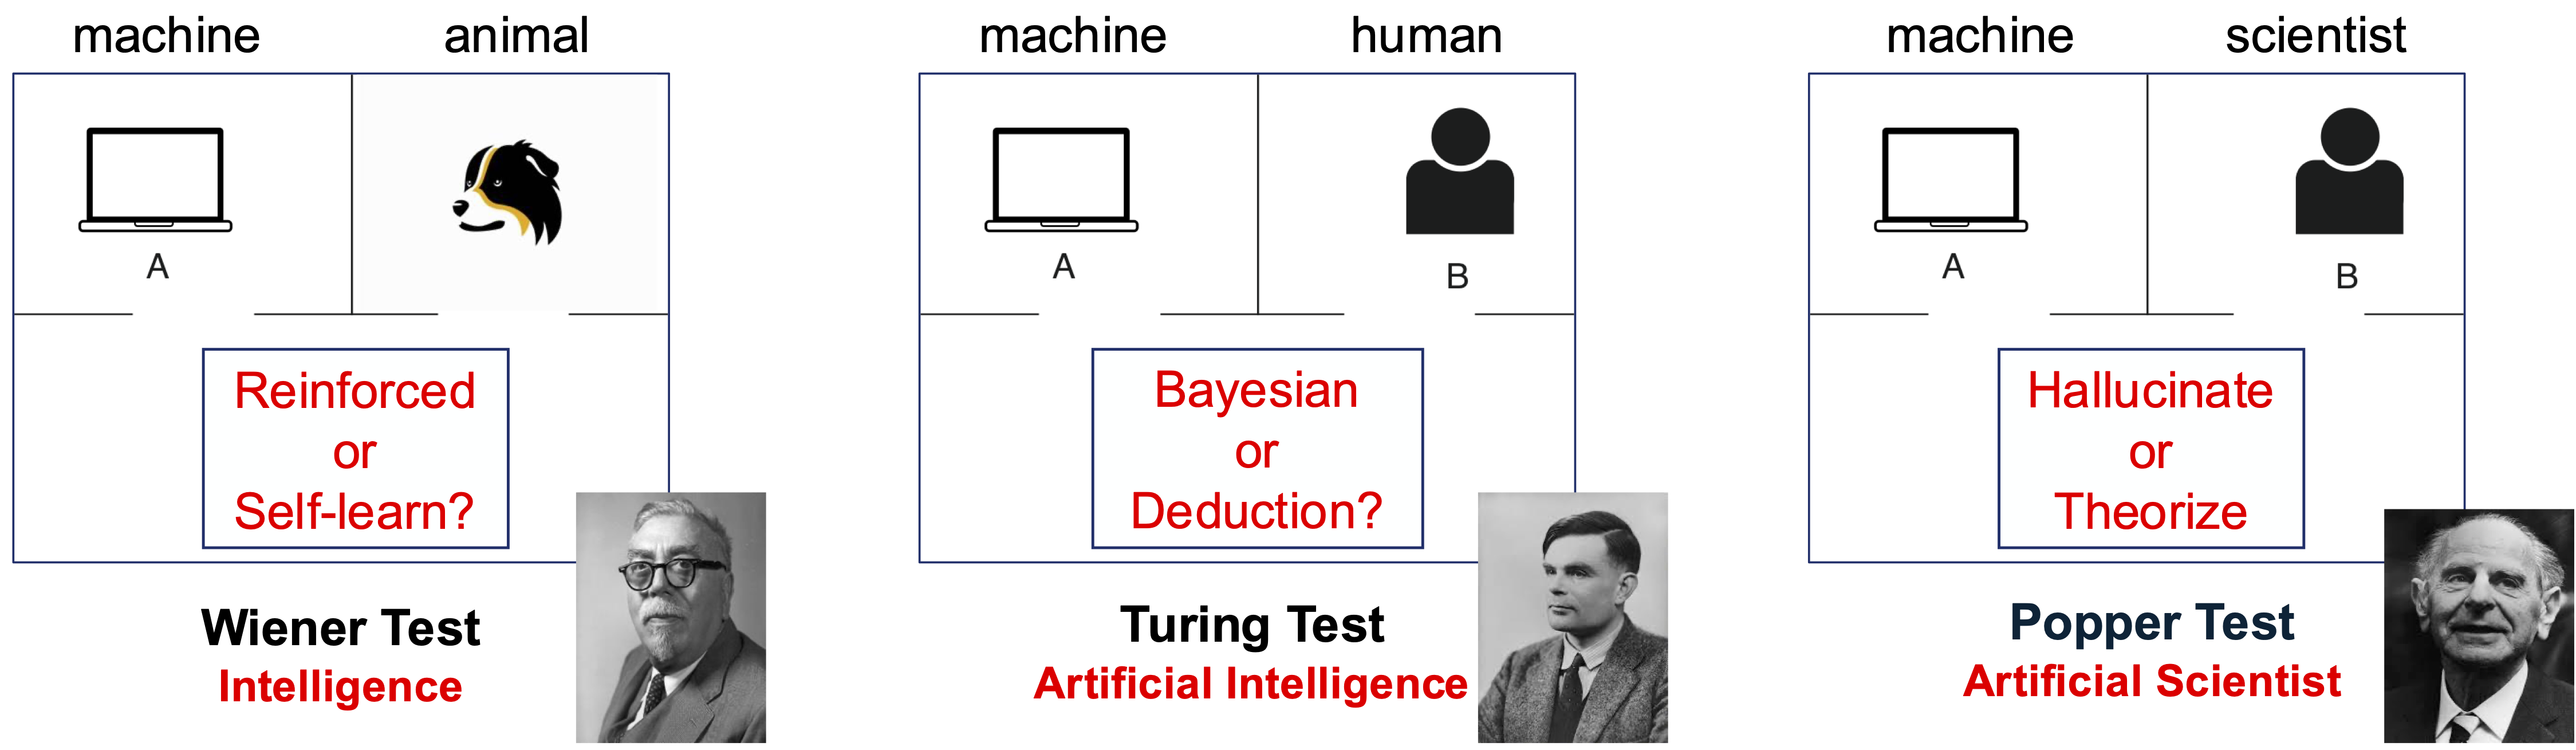
\includegraphics[width=0.95\linewidth]{\toplevelprefix/chapters/chapter8/figs/tests.png}
    \caption{针对不同层次或类型智能能力的三种测试:维纳测试、图灵测试和波普尔测试。}
    \label{fig:three-tests}
\end{figure}

图\ref{fig:three-tests}说明,可能至少应该有三种不同类型的测试来评估和区分不同类型的智能能力:
\begin{enumerate}
    \item {\em 诺伯特·维纳测试:} 评估一个系统是能够自我改进和发展新知识,还是仅仅通过强化或监督学习接收信息;
    \item {\em 艾伦·图灵测试:} 评估一个系统是能理解抽象知识,还是仅仅学习其统计规律并用于贝叶斯推理;
    \item {\em 卡尔·波普尔测试:} 评估一个系统是否能够通过形成和验证基于自洽性的新理论来探索新知识。
\end{enumerate}
我们相信,对于这样的评估方法,评估者不应是人类,而应是一个科学上合理的协议和过程。



正如我们在全书中所见,\textit{压缩}在学习中扮演了最基础的角色。它是识别(经验)数据分布和组织其中编码的信息的支配性原则和统一机制。在很大程度上,它解释了过去十几年“人工智能”的大部分实践。这里的“人工”一词主要意为“人造的”。未来研究的一个悬而未决的问题是,\textit{仅凭压缩}是否足以实现上述所有更高阶的智能能力?
\begin{quote}
\begin{center}
        {\em 压缩是否就是一切?}
\end{center}
\end{quote}
抽象、因果推理、逻辑推理以及假设的生成和检验,是否是压缩的某种延伸或极端形式?通过压缩来识别(经验)数据分布与提取高阶理论或定律之间是否存在根本性的区别?正如哲学家卡尔·波普尔曾经指出的:
\begin{quote}
    \begin{center}
    {\em “科学或可被描述为系统性地化繁为极简的艺术。”}
    \end{center}
\end{quote}
在很大程度上,科学可以被视为最高级的智能形式,因此也是智能中真正的“人工”部分。这里的“人工”一词意指(受过科学启迪的)人类所独有的理解与创造能力。我们相信,揭示并理解这种更高阶智能背后的数学原理和计算机制,将是科学、数学和计算共同的终极归宿!

\end{document}
